%\documentclass{sig-alternate}
%\documentclass[]{sig-alternate-05-2015}
%\documentclass[10pt, conference, compsocconf]{IEEEtran}
\documentclass[10pt, conference]{IEEEtran}
\IEEEoverridecommandlockouts      % enable the \IEEEpubid command for the 'conference' class

\usepackage{amsmath}
\usepackage{amsthm}
\usepackage{accents}
\newcommand*\underdot[1]{%
  \underaccent{\dot}{#1}}
\usepackage{mathtools}
\DeclarePairedDelimiter\ceil{\lceil}{\rceil}
\DeclarePairedDelimiter\floor{\lfloor}{\rfloor}
\usepackage{mathrsfs}
\usepackage{times}
\usepackage{multirow}
\usepackage{enumitem}
\usepackage{epsfig}
\usepackage{subfigure}
\usepackage{amsfonts}
\usepackage{amssymb}
\usepackage{graphicx}
\usepackage{url}
%\usepackage{cite}
\usepackage{psfrag}
\usepackage{array}
\usepackage{comment}
\usepackage{mdwmath} % part of Mark Wooding's powerful
\usepackage{mdwtab}  % tools for math, tables, ...
\usepackage{bm} % for the bold font Greek symbols in math mode
\usepackage{color}
%\usepackage[noend]{algorithmic}
\usepackage[noend]{algpseudocode}
\makeatletter
\usepackage{multirow}
\usepackage{algorithm}
\usepackage{xspace}
%\usepackage{flushend}  <-- Bear, ACM do not like balanced last page
\usepackage{natbib}  % for small reference font size
\def\bibfont{\footnotesize}
\setlength{\bibsep}{0.0pt}

%\usepackage{float}
%\usepackage{natbib}  % for small reference font size
%\def\bibfont{\scriptsize}
%\setlength{\bibsep}{0.0pt}
%\usepackage{enumitem}
%\setlist{nolistsep}

% INFOCOM specific space saving tips from Bo
%\renewcommand{\baselinestretch}{0.990}
% place it after 'documentclass' for shrinking line space. Default is 1. 0.92 is the minimum acceptable by INFOCOM
%\usepackage[left=0.625in,right=0.625in,top=0.75in,bottom=1in]{geometry}
% this sets the margins of the 3 sides. The numbers are the minimum acceptable by INFOCOM

\newtheorem{thm}{Theorem}
\newtheorem{cor}{Corollary}
\newtheorem{lem}{Lemma}
\newtheorem{dfn}{Definition}
\newtheorem{pbm}{Problem}
\newtheorem{claim}{Claim}

%\remove copyright box
%\makeatletter
%\def\@copyrightspace{\relax}
%\makeatother


\begin{document}
\sloppy

\title{
Streaming Scalable Video Sequences with Media-Aware Network Elements Implemented in P4 Programming Language
}

\author{ 
\IEEEauthorblockN{Chao-Wen Chen$^1$, Cheng-Hsin Hsu$^2$}
\vspace{2pt}
\IEEEauthorblockA{$^1$Department of Computer Science, National Tsing Hua University, Taiwan}
}

\maketitle

\begin{abstract}
\end{abstract}

\begin{IEEEkeywords}
Scalable video streaming, media-aware network element, software-defined network, rate-distortion optimization
\end{IEEEkeywords}

\section{Introduction} \label{sec:introduction}

In recent years, people are getting used to rely on Over-The-Top (OTT) 
services such as Skype, Facebook, Youtube, Netflix, etc. 
Among these services, video streaming is one of the services which 
consumes the most network resources. Video streaming needs more and more bandwidth because receivers prefer higher video quality than before, and thus incur high traffic amount on the best-effort Internet. Turns out streaming high quality video with less network resources becomes much more important.

{\em Scalable Video Coding (SVC) }is one of solutions for network congestion. Each of the SVC sequences contains a header, a base and multiple enhancement layers. The header stores the information that how the decoder should recognize those packets, and the base layer consists the elementary information of that particular frame. Enhancement layers are all rely on the low layers to decode. For example, enhancement layer 1 can be decode only if receiver receive the base layer and enhancement layer 2 can be decode only if receiver receive the enhancement layer 1. Furthermore, the encoder will encode the discardability into the packetize header. Therefore, We can drop the discardable packets without affecting its decodability in the middle-box of the Internet. The dynamic decisions on which video packets to drop can be sub-optimally done by streaming servers or clients without the global knowledge of the Internet. The better way to approach is through {\em Media-Aware Network Elements (MANEs)}, which are switches with knowledge of packets header. However, changing the normal switches into MANEs is quite difficult and thus not likely to happen. Fortunately, with recent advances in {\em Software-Defined Networking (SDN)} and {\em Network Function Virtualization (NVF)}, network switches are much more programmable, and make collaborative MANEs into reality. 

In the following sections, we will introduce every tools we are going to use and evaluate the results of our experiments among each algorithm we designed.
\begin{figure}[tbh]
		\centering
		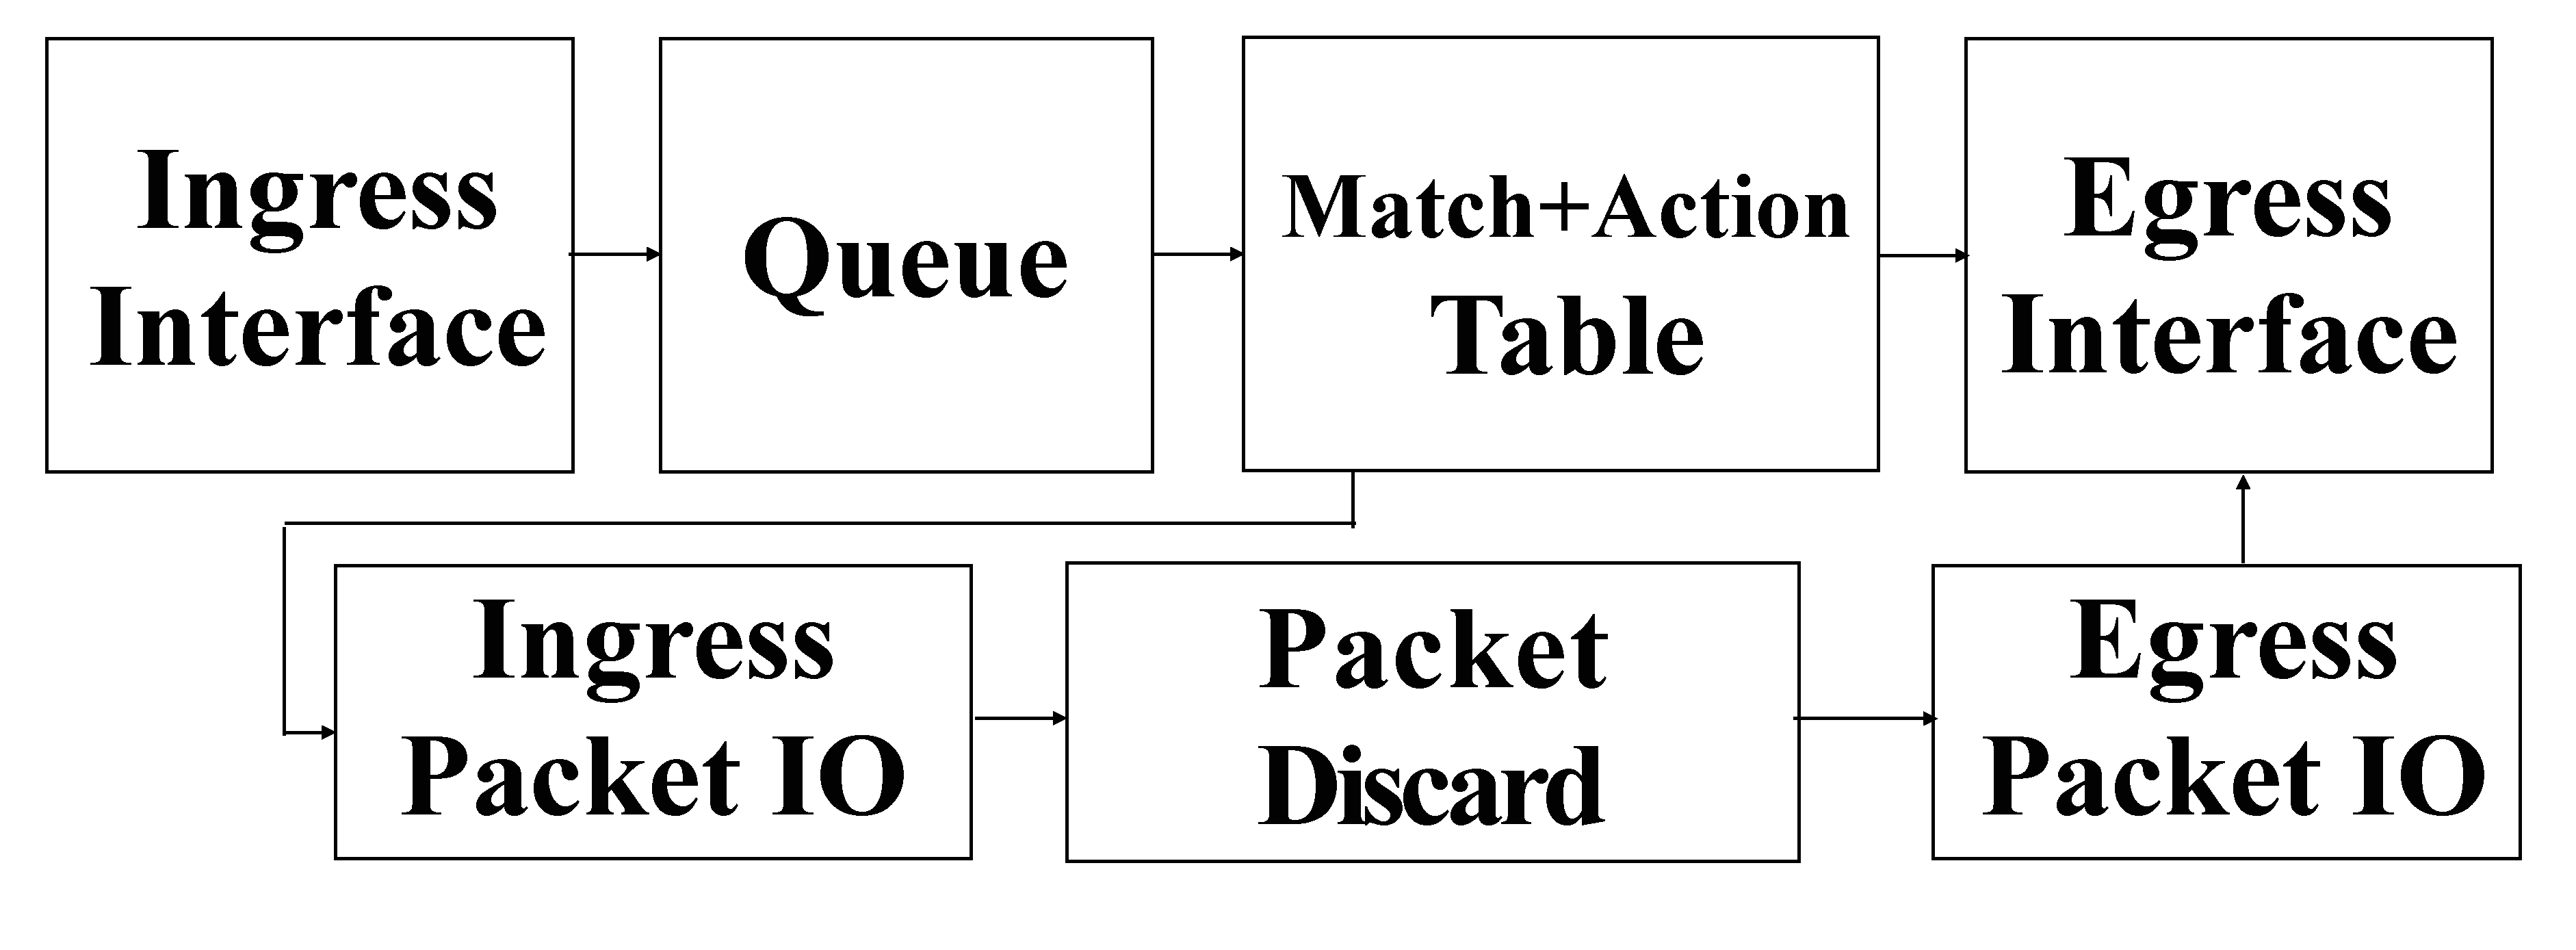
\includegraphics[width=.24\textwidth]{fig/MANE_1.eps}
		\caption{Packet processing in a P4-based MANE.}
		\label{MANE}
\end{figure}

\section{Media-Aware Network Element} \label{sec:mane}
\begin{comment}
{\em We show how to intelligently drop scalable video
packets to retain streamed video quality, when bandwidth is insufficient and
dynamic.} We consider three {\em packet discarding logics}: (i) tail, (ii)
enhancement-layer (EL), and (iii) rate-distortion optimized (RDO). Tail always
drops the last packet in the queue, while EL only drops the enhancement-layer
packets when needed. The advantage of tail logic is simplicity, while EL logic
ensures the decodability of received videos. RDO logic is more comprehensive,
as it takes the nonlinear nature between distortion and bitrate into
considerations. By dropping the packets with the least distortion and bitrate
ratio, RDO logic aims to minimize the negative impacts of dropping packets on
video quality.



We have implemented a MANE in P4 programming language~\cite{BDGI+14}. Fig.~\ref{MANE} shows
how the P4-based MANE processes the packets. First, we define the header formats
and parsers, which allow us to understand the structure of individual packets.
We use the information in headers to check if packets are valid.
Next, we define tables to describe how the header
fields should be matched in the match+action stage.  The control program pushes
the packets into one of the queues based on their header fields.  It starts to
throttle the ingress packets when the queue occupancy exceeds a
admin-specified threshold. More specifically, the {\em packet discard logic} picks and
drops some packets, in order to maintain high overall video streaming quality; 
other packets are forwarded.

% Bear, may be reused later
\begin{comment}
Programming Protocol Independent Packet Processors (P4) Language is a high-level language for constructing a packet-control system on a specific switch. It will first define parser information, control program, and flow table. Next, it defines actual packet parser, ingress control, egress control. The are differences between P4 and traditional SDN,  SDN controller can only process traditional packets but P4 can define our own packet format and decide what action should be made.

\begin{figure}[h]
		\centering
		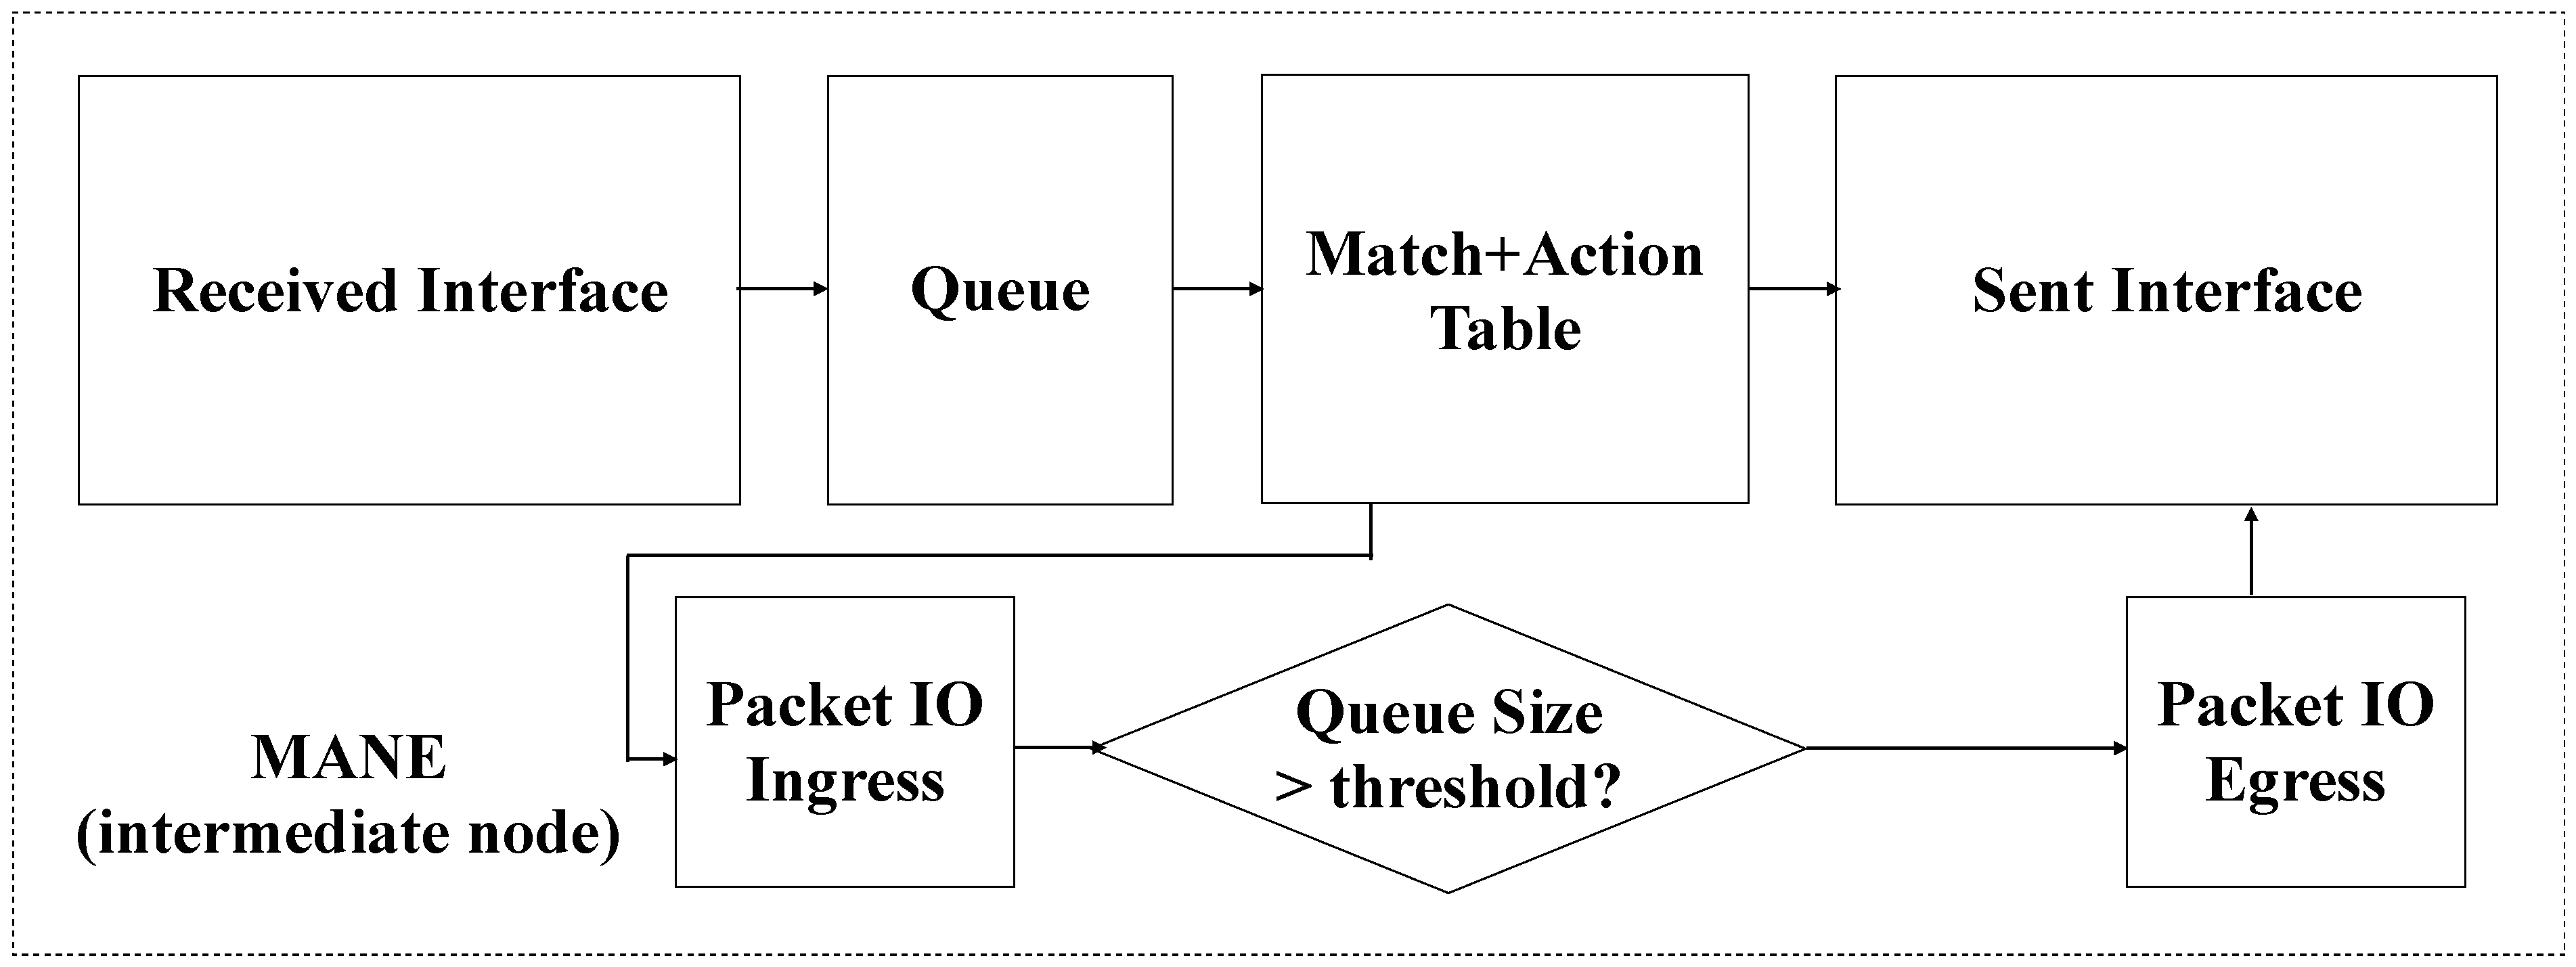
\includegraphics[width=5cm]{fig/network.eps}
		\caption{MANE Structure}
		\label{scenario_1}
\end{figure}

Layered video coding helps to supply multiple streams to meet the requirements of heterogeneous network environment. Scalable video coding(SVC) is a extension of traditional H.264/MPEG-4 AVC. It provides three mainly characteristic, temporal scalability, spatial scalabilility and SNR scalability. With these characteristics, SVC video transmission could be more adaptable in variety QoS demands. 

Media Aware Network Element(MANE) is an intermediate node between server and client. The MANE managers the SVC packets in the middle of the network. In this paper, our goal is to implement a P4 switch to act as a MANE. We define the packet format and how to handle packets in P4 switch. Next, we drop some of these packets if our queue is growing bigger and bigger. In scalable video steaming,the whole frame cannot be decode if the base layer is dropped. So this paper wants to keep more base layers as possible. However, we should maintain the video quality simultaneously. There are three algorithms to be considered.
\begin{itemize}
\item Tail drop
\item Base Only
\item Rate Distortion Optimization(RDO)
\end{itemize}

The traditional algorithm to handle network congestion is tail drop. It's similar to a FIFO queue. The biggest advantage is it's simple implementation. Because of the limit of queue size, switch will drop the incoming packet if the queue is already full. If tail drop happened. Server will be announced and adapt sending rate. Since we know that layered video coding only needs base layer to be decoded, we can simply drop all the enhancement layer to solve network congestion. The second algorithm drops all enhancement layer no matter how full the queue is. In other words, client receives base layer only. RDO is used in today's single layer video coding. It's target is minimize the distortion D for a given rate R. We can find some information in packet header to calculate the distortion in runtime. Then we combine early detected policy. If the queue size is bigger than threshold, we start to drop the packet with largest distortion and never drop a base layer packet unless the queue is complete full. With this algorithm, we can guarantee that the base layer will always be forwarded and optimize layered video streaming.

Combining P4 switch and MANE, we can reduce the delay and provideSince we know that layered video coding only needs base layer to be decoded, we can simply drop all the enhancement layer to solve network congestion.  same video quality using less network resources. SDN can configure the best path to stream videos. Furthermore, if the network is unreliable, SDN and administrators can take control to that situation automatically and remotely. In the future, we may not need MANE anymore, we could use SDN and P4 switch to gain a better network environment.

\end{comment}

\begin{figure}[tbh]
		\centering
		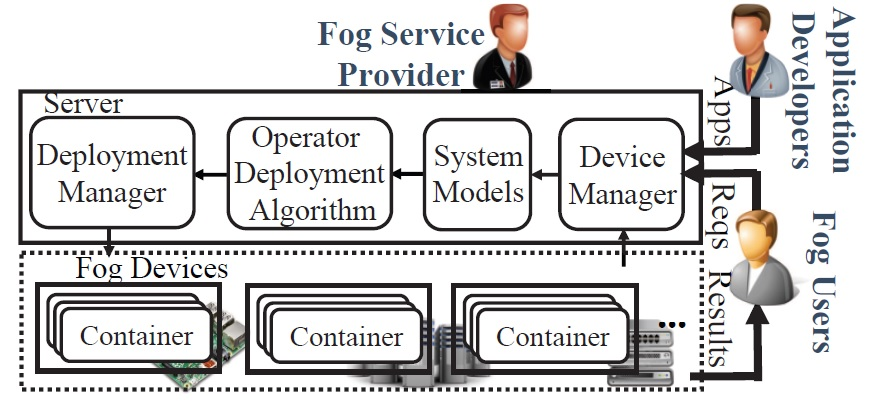
\includegraphics[width=0.40\textwidth]{fig/architecture.eps}
		\caption{High-level system architecture with a network of MANEs.}
\vspace{-0.1cm}
		\label{architecture} 
\end{figure}

\section{System Architecture} \label{sec:architecture}

%The considered system is composed of an ONOS controller, a video server, multiple video clients, and several MANEs as shown in Fig.~\ref{architecture}. The ONOS controller forms a control plane disassociated from data plane among P4 switches. Using the knowledge on the network topology and available resources, the ONOS controller determines the best routes from servers through MANEs to clients. Once the streaming starts, each MANE drops the scalable video packets when necessary.
%
%The life cycle of the video streaming sessions is as follows. First, the receiver sends a request to the server, and the server sends the encoded video streams through the MANEs. During transmissions, the ONOS controller communicates with all MANEs to set up the outgoing port for packets. When the network topology changes, the ONOS controller informs every MANE for the alternative paths immediately. The ONOS controller may also fine-tune the video quality levels of different users for optimal overall quality.


\section{Experiment Setup} \label{sec:setup}

We design a system using the tools we introduce above including SVEF, bmv2, and P4. Because of the limit of fund, we use bmv2 inside mininet and test our three drop logics. Three scenarios are designed to compare the difference among these drop logics. 

We use real H.264/SVC video sequences in our experiments, and these scenarios are done in mininet with software MANEs (running {\em bmv2}~cite{bmv2}) and virtual hosts.
In these scenarios, we would like to see the characteristic of P4 and our contribution. These three scenarios are described below:

Fig. ~\ref{scenario1}, ~\ref{scenario2} and ~\ref{scenario3} are scenarios we use to evaluate tail and EL logics. The RDO logic will be test only in scenario 3.

\begin{figure}[tbh]
	\centering
	\begin{minipage}[t]{0.24\textwidth}
	\centering
	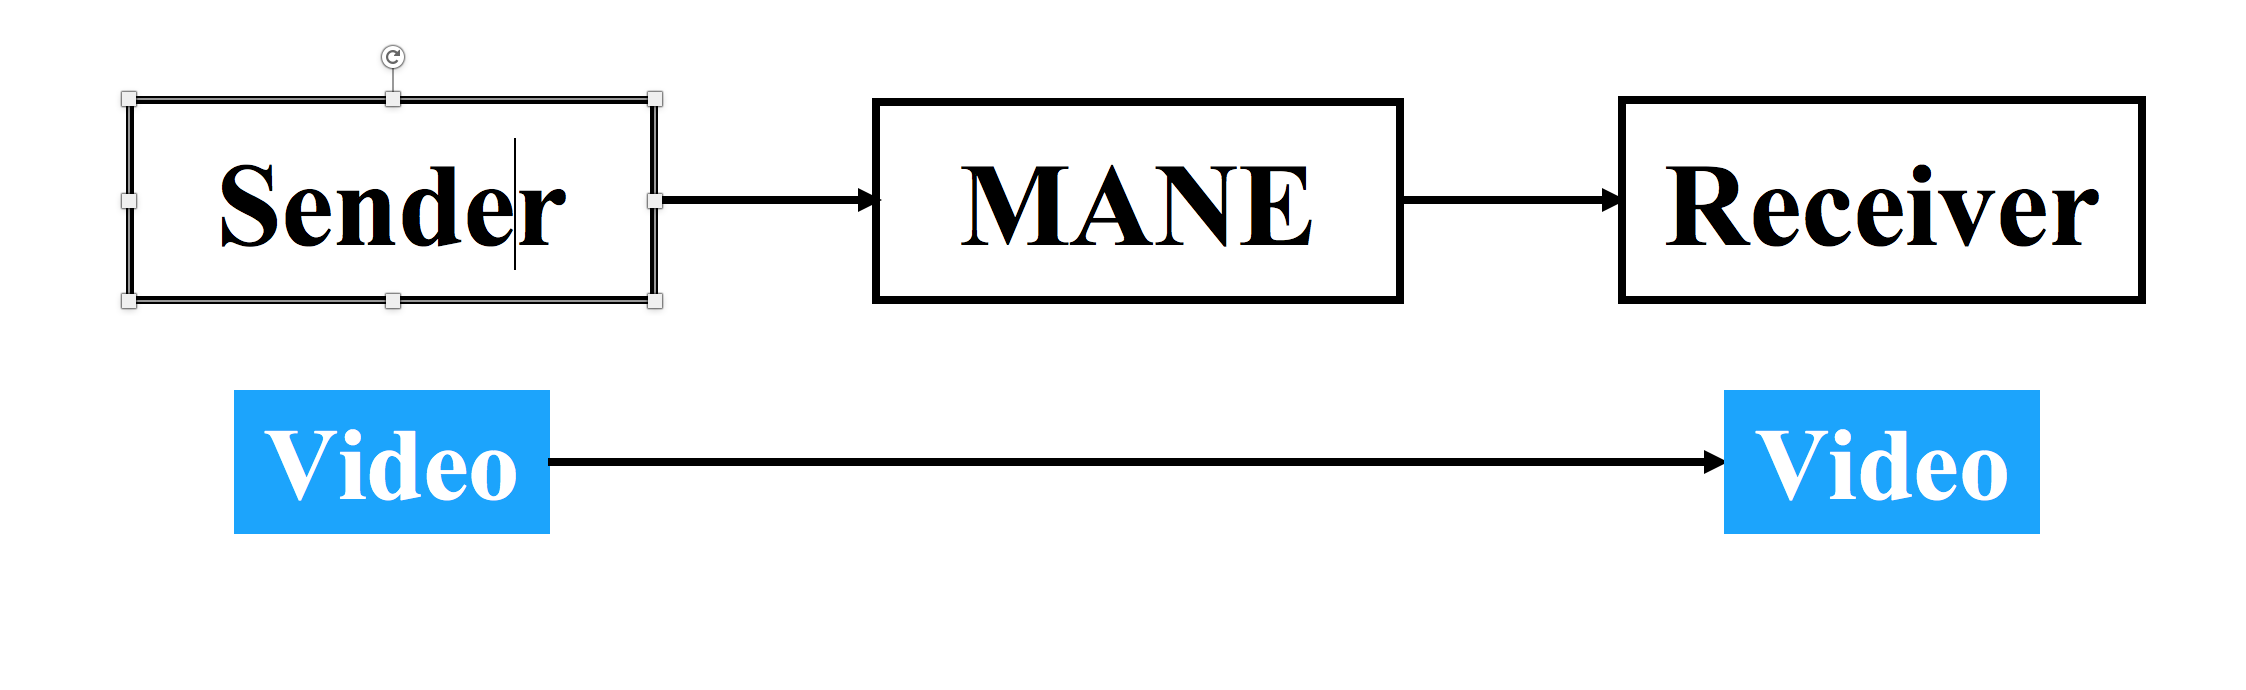
\includegraphics[width=\textwidth]{fig/scenario1.png}
	\caption{Testbed topology (scenarios 1).}
	\label{scenario1} 
	\end{minipage}
	\hfill\begin{minipage}[t]{0.23\textwidth}
	\centering
	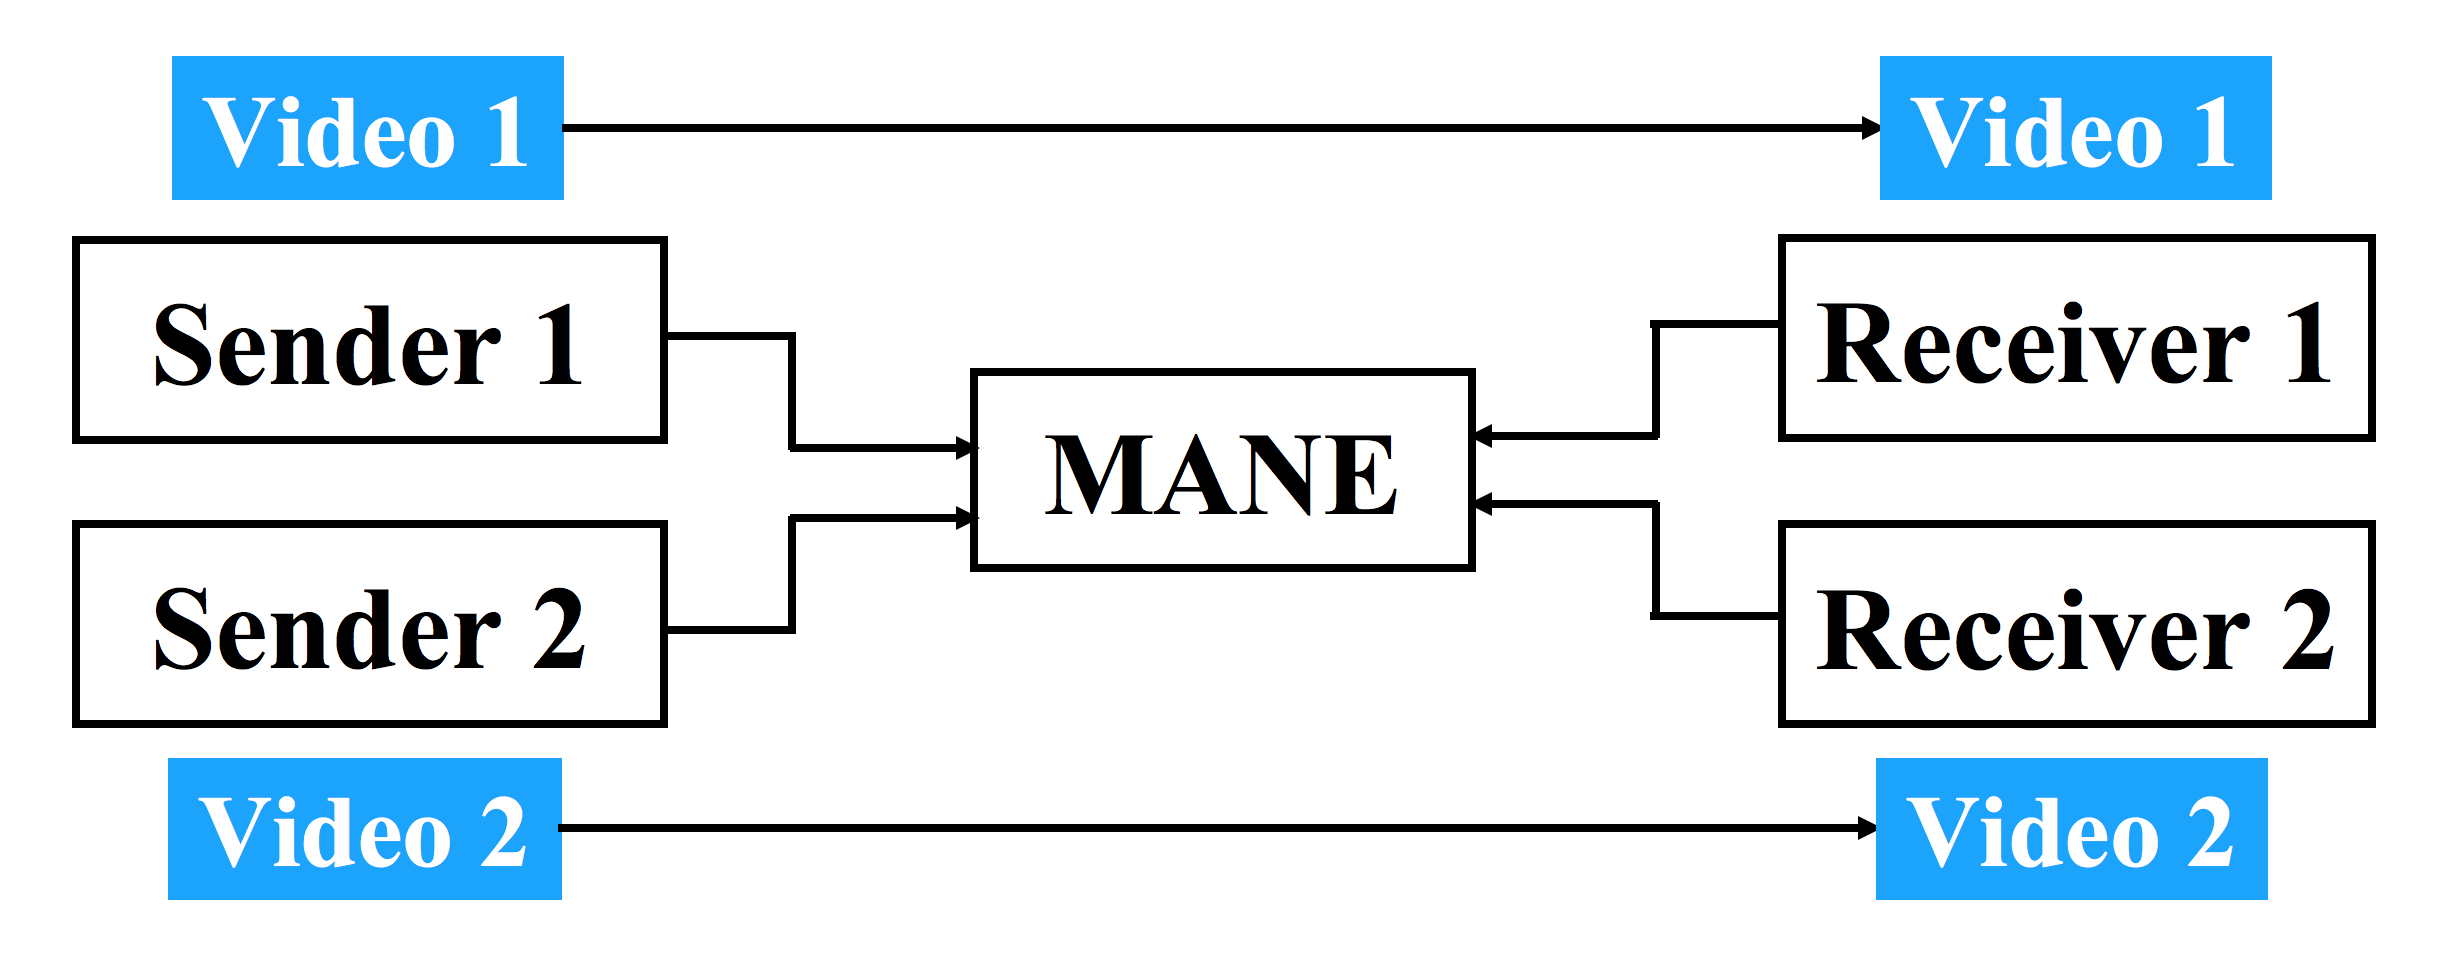
\includegraphics[width=\textwidth]{fig/scenario2.png}
	\caption{Testbed topology (scenario 2).}
	\label{scenario2} 
	\end{minipage}
	\vspace{-0.1cm}
\end{figure}

\begin{itemize} 
	\item {\bf Intelligent packet drops of a single video stream.}
	We construct a simple network with a sender, a controller, a MANE, and a receiver. Scenario 1 is the simplest topology. It consists of one sender and one receiver streaming one video. In this scenario, we want to observe the drawbacks of tail logic and see if EL logic can reduce network congestion by eliminate undecodable packets. The mininet bandwidth on the link is varied over time by scripts. In the MANE, we implement tail, EL, and RDO logics, and compare their performance. 

	\item {\bf Optimal packet drops across multiple video streams.}
	Scenario 2 is has four hosts with two sender and two receiver streaming two videos in mininet. In this scenario, we can use twice of buffer than scenario 1 because packets should be forwarded to different hosts and pushed into different buffer. In the MANE, we also implement three drop logics, and We can imagine that the result of scenario 1 and 2 would be very similar.

	\item{\bf Eliminate undecodable packets in less buffer}
	Scenario 3 shown in Fig.~\ref{scenario3} is the most challenging one. It contains one sender and one receiver streaming two videos in the same time. In this scenario, two streaming flows could affect each other since there is still exist a small time gap between them. When our P4-based MANE receive packets. It could push packets belong to one of the streaming flow but drop the other since the size of buffer exceed threshold after pushing that packet. 

\end{itemize}

\begin{figure}[tbh]
	\centering
	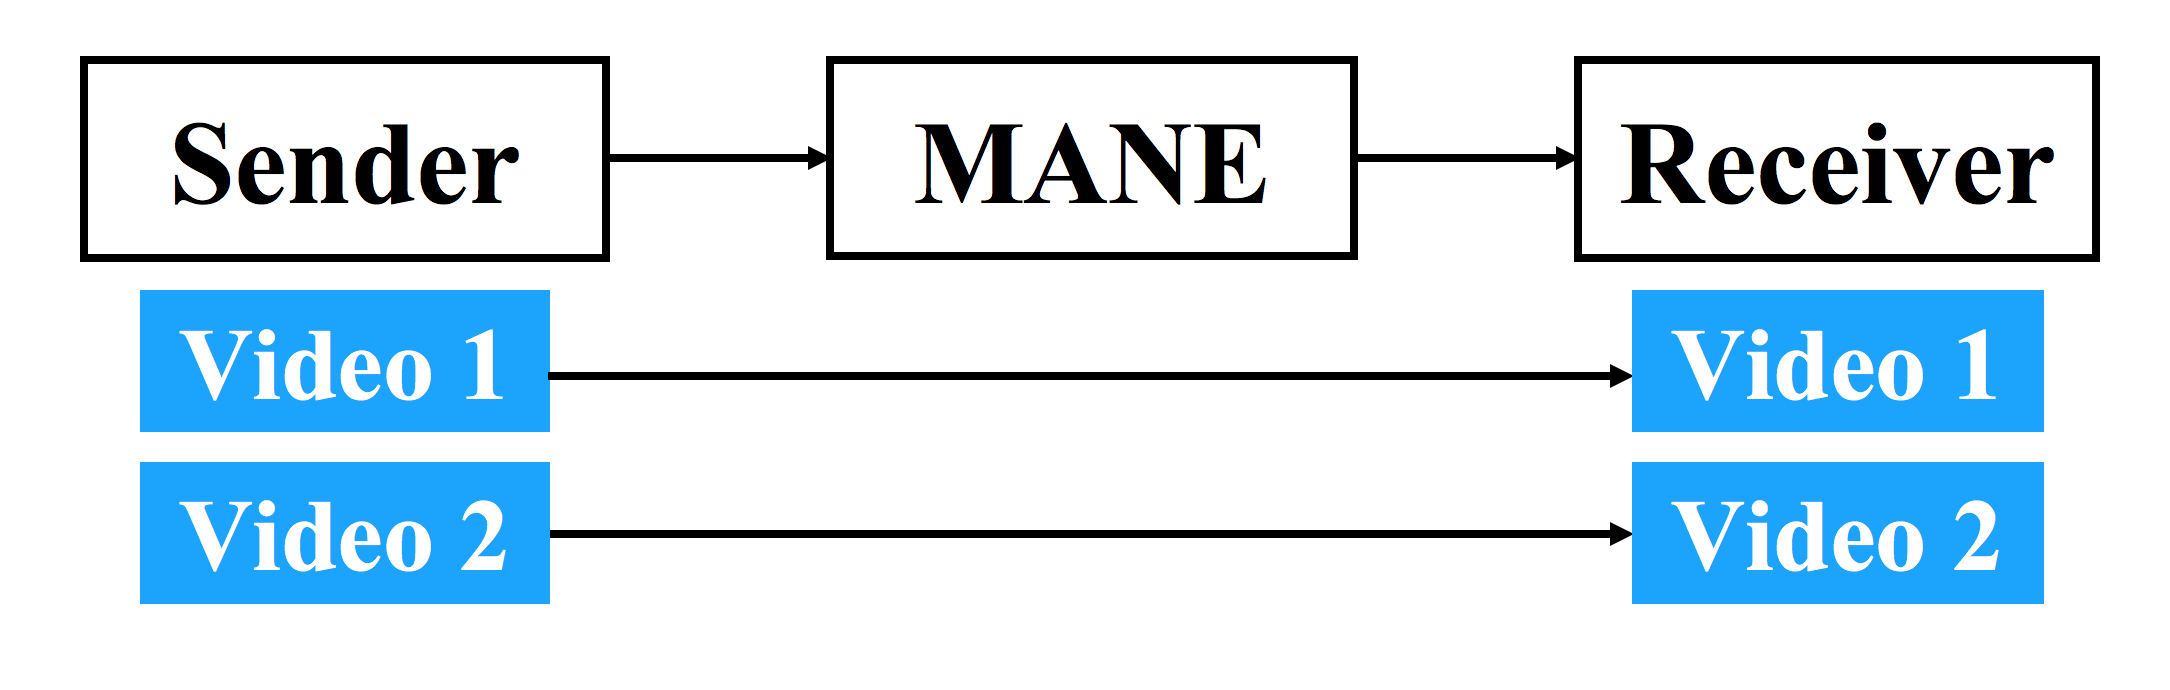
\includegraphics[width=.50\textwidth]{fig/scenario3.png}
	\caption{Testbed topology (scenarios 3).}
	\label{scenario3} 
\end{figure}

Among these scenarios. We try to limit the bandwidth between all of the links using tclink of mininet. However, this approach simply drops all packets at the backend of mininet if the throughput exceeds our administrate-set bandwidth without any signal or error exception. Even the bmv2 itself doesn't know if the packet is transmit by the attached interface. We follow the instructions given by the author of bmv2, limit the bandwidth by limit the packet sending rate. Through this approach, we can limit the bandwidth by quantities of packet instead of throughput. We need this because our drop logics will decide which packet to drop instead of dropping partition of the packet content.

%{\bf Preliminary evaluation.}
%To evaluate the performance of RDO, we use the following Quality of %Experience (QoE) measurements to compare tail drop, base-only and RDO %algorithms and compare the RDO with the general switches as well.

%\begin{itemize}
%\item {\bf Network latency}  Since more and more people watch video online, network latency is an important factor that impact users on watching videos.
%\item {\bf Network bandwidth} Videos nowadays usually have large resolutions, especially the presence of 4K videos. However, it is difficult to upgrade the network bandwidth on network links, which are usually fixed. Thus, we evaluate our algorithms and expect RDO can   
%\item {\bf Video quality}
%\end{itemize}

\begin{comment}
\section{Conclusion and Outlook} \label{sec:conclusion}

We have demonstrated the feasibility of realizing MANE for
scalable video streaming using P4 programming language. Through the high
programmability offered by software-defined networks, we show how optimally
dropping scalable video packets improves the streaming quality, while many
other optimization approaches are possible in the future. For example, 
video and non-video
Internet services can be managed in a Quality-of-Service fair way, and popular
video packets can be proactively or reactively cached.

\end{comment}


%\section*{Acknowledgements}
%This work was partially supported by the Ministry of Science and Technology of Taiwan under the grant \#106-2221-E-007-101.
%\begin{figure}
%	\centering
%	\includegraphics[width=0.7\linewidth]{noms18Demo}
%	\caption{}
%	\label{fig:noms18demo}
%\end{figure}

%{\small
\bibliographystyle{abbrv}
\bibliography{./ref}
%}
\end{document}

